\chapter{Nonlinear dynamical systems on the plane}
For this chapter the general setup will be 
\begin{align}
	\dot{x} = f(x);\quad x \in \mathbb{R}^{2};\quad f\in C^1.
\end{align}
\section{One degree of freedom conservative mechanical systems}
Write $x = 
\begin{pmatrix}
	x_1 \\ x_2
\end{pmatrix}
$, with $x_1$ denoting the position and $x_2=\dot{x}_1$ denoting the speed. The total mechanical energy is given by $E(x) = \frac{1}{2}mx_2^2  + V(x_1)$, with the mass $m$ and the potential function $V$. Newton's law then gives the equations of motion 
\begin{align}
	m \ddot{x}_1 = -\frac{dV(x_1)}{dx_1} \implies 
	\begin{dcases}
		\dot{x}_1 = x_2 \\
		\dot{x}_2 = - \frac{1}{m} \frac{dV(x_1)}{dx_1}.
	\end{dcases}
\end{align}
All of the forces derive from a time-independent potential. The energy is a first integral (conserved quantity of such systems), i.e.
\begin{align}
	\frac{d}{dt}E(x(t)) = \frac{\partial E}{\partial x_1}\dot{x}_1 + \frac{\partial E}{\partial x_2}\dot{x}_2 = 0.
\end{align}
Therefore on any given trajectory $x(t)$ the energy $E(x(t))=E_0 $ is constant. Hence we can derive an explicit equation for the velocity along a trajectory which suppresses the time dependence
\begin{align}
	x_2 = \pm \sqrt{\frac{2}{m}(E_0 -V(x_1))}.
\end{align}
This leads to multiple consequences for these systems
\begin{enumerate}
	\item Trajectories form symmetric pairs (w.r.t. the $x_1$-axis) of the same energy.
	\item There is a clockwise orientation for trajectories due to 
		\begin{align}
			\dot{x}_1 = x_2 \implies
			\begin{cases}
				x_2>0 \implies x_1  \textrm{ increases} \\
				x_2 <0 \implies x_1  \textrm{ decreases} .
			\end{cases}
		\end{align}
		This is shown graphically in Fig. \ref{fig:mech_clock_orient}.
		\begin{figure}[h!]
			\centering
			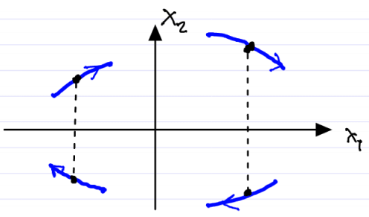
\includegraphics[width=0.4\textwidth]{figures/ch4/1mech_clock_orient.png}
			\caption{The clockwise orientation of trajectories in 1 degree of freedom conservative mechanical systems.}
			\label{fig:mech_clock_orient}
		\end{figure}
	\item Local minima of the potential give rise to a center fixed point surrounded by closed orbits. The minima $x^{*} $ is a fixed point if $x^{*}_2 = 0$ (which occurs if $V(x^*_1) = E_0$) as $\dot{x}_2 \propto V'(x^{*}_1) = 0 $. The trajectories of the closed orbits can be found using $x_2 = \pm \sqrt{\frac{2}{m}(E_0 - V(x_1))}$. Such a local minima fixed point surrounded by closed orbits is shown in Fig. \ref{fig:mech_loc_extrem}.
\begin{figure}[h!]
	\centering
	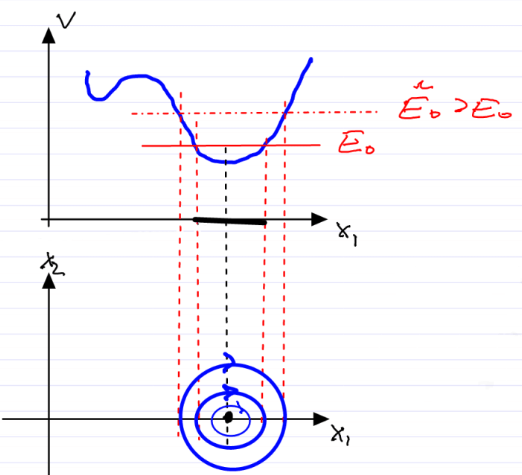
\includegraphics[width=0.47\textwidth]{figures/ch4/2mech_orbits_minima.png}
	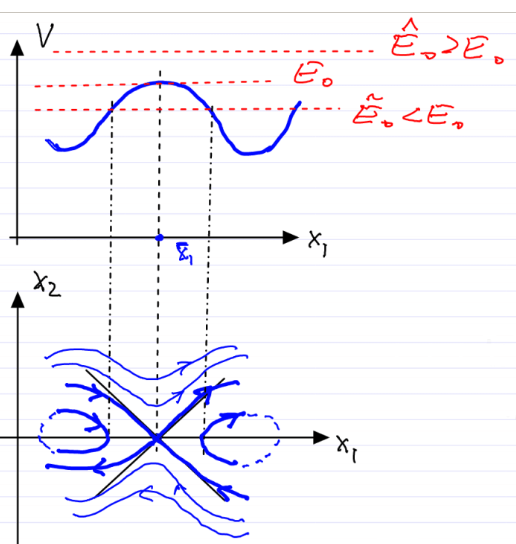
\includegraphics[width=0.39\textwidth]{figures/ch4/3mech_orbits_maxima.png}
	\caption{Left: Closed orbits around the fixed point at the local minima of the potential function. Right: The saddle type fixed point at the local maxima of the potential. The clockwise orientations comes from consequence (ii).}
	\label{fig:mech_loc_extrem}
\end{figure}
\item At local maxima of the potential saddle type fixed points arise. The maxima $x^{*}$ is a fixed point if $x^{*}_2=0 $ (which occurs if $V(x^*_1)=E_0$) as $V'(x^{*}_2)=0$. The velocity can be approximated as follows
	 \begin{align}
		 x_2 &= \pm \sqrt{\frac{2}{m}(E_0 -V(x_1))} \\
		     &= \pm \sqrt{\frac{2}{m}} \sqrt{\underbrace{(E_0 - V(x^{*}_1))}_{=0} - \underbrace{V'(x^{*}_{1})}_{=0}(x_1 - x^{*}_1) - \frac{1}{2}\underbrace{V''(x^{*}_1)}_{<0}(x_1 - x^{*}_{1})^2 + \mathcal{O}((x_1 - x^{*}_1)^3)} \\
		     &=\pm \sqrt{\frac{2}{m}}\sqrt{-\frac{V''(x^{*}_1)}{2}}\left|x_1 - x^{*}_1\right| +  \textrm{higher order terms} .
	\end{align}
The behavior is sketched in Fig. \ref{fig:mech_loc_extrem}
\item A local minima has local maxima to the left and right, unless $V$ is monotonously nondecreasing to infinity. Then we have two cases to differentiate. One where the local maxima are at the same level, and the other where one local maxima is not as large as the other (or in one direction $V$ monotonously increases towards infinity). These two cases are illustrated in Fig. \ref{fig:mech_limit_case}. 
	\begin{figure}[h!]
		\centering
		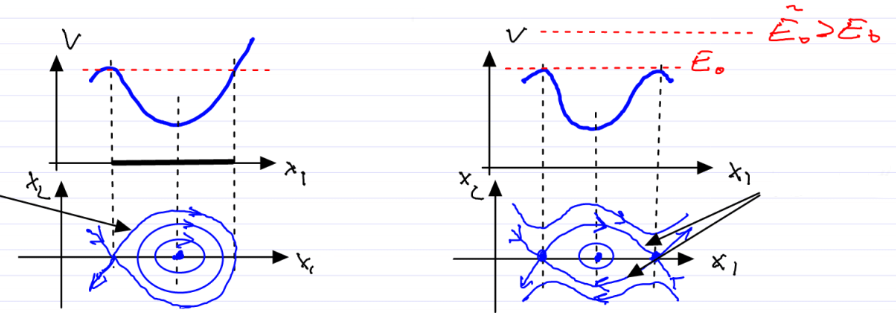
\includegraphics[width=0.9\textwidth]{figures/ch4/4mech_limit_case.png}
		\caption{Left: One maxima is lower than the other (or $V$ is nondecreasing towards infinity on the right). The black arrow denotes a \emph{homoclinic orbit}. Right: Each maxima is at the same level. The black arrows denote \emph{heteroclinic orbits}.}
		\label{fig:mech_limit_case}
	\end{figure}
	
\end{enumerate}

These consequences are illuminated in a basic example.
\begin{ex}[The Duffing oscillator]
Let the equation of motion be given by
\begin{align}
\ddot{x}-x+x^3=0;\quad x_1=x;\quad x_2=\dot{x}.	
\end{align}
Therefore we get the first order ODE
\begin{align}
	\begin{dcases}
		\dot{x}_1 = x_2 \\
		\dot{x}_2 = x_1 - x_1^3 = - V'(x_1)
	\end{dcases}
	\implies E(x) = \frac{1}{2}x_2^2+ V(x_1) = \frac{1}{2}x_2^2 + \left( - \frac{1}{2}x_1^2 + \frac{1}{4}x_1^4\right).	
\end{align}
The full phase portrait of two homoclinic orbits is shown in Fig. \ref{fig:duffing_phase_portrait}.
\begin{figure}[h!]
	\centering
	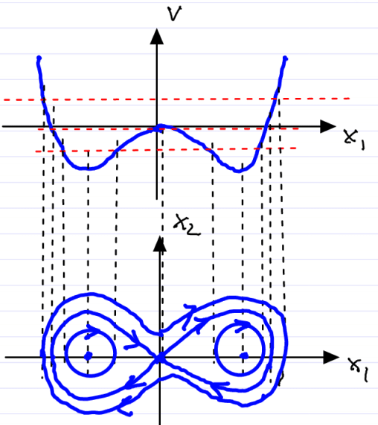
\includegraphics[width=0.4\textwidth]{figures/ch4/5duffing_phase_portrait.png}
	\caption{Phase portrait of the Duffing oscillator using the potential $V$.}
	\label{fig:duffing_phase_portrait}
\end{figure}

\end{ex}

\section{Global behavior in two dimensional autonomous dynamical systems}
Consider the following dynamical system
\begin{align}
	\dot{x} = f(x);\quad x \in \mathbb{R}^{2};\quad f \in C^1.
\end{align}
Further assume that solutions exist for all times, therefore there exists a unique solution $x(t; x_0)$ for all $t \in \mathbb{R}$ such that $x(0;x_0)=x_0$. Next, a few definitions are introduced enabling a deeper exploration of such systems.

\begin{definition}
	An \emph{$\omega$-limit point} of $x_0$ is a point $p \in \mathbb{R}^{2}$ if there exists a monotone increasing unbounded sequence of times $\{t_i\}_{i=1}^{\infty}$ with $t_1 \geq 0$ such that 
	\begin{align}
		\lim_{i\to \infty}x(t_i;x_0)=p.
	\end{align}
\end{definition}

\begin{definition}
	An \emph{$\alpha$-limit point} of $x_0$ is a point $q \in \mathbb{R}^{2}$ which is an $\omega $ limit point in backwards time. 
\end{definition}

\begin{definition}
	The \emph{$\omega $-limit set} of $x_0$, denoted $\omega(x_0)$ is the set of all $\omega$-limit points of $x_0$.
	The \emph{$\alpha $-limit set} of $x_0$, denoted $\alpha(x_0)$ is the set of all $\alpha$-limit points of $x_0$.
\end{definition}
\begin{remark}[]
	Note that $\omega(x_0)$ and $\alpha(x_0)$ is the same for all $x_0 $ along a given trajectory, thus limit sets can be associated with full trajectories.
\end{remark}
\begin{ex}[Examples of limit sets]
	Below (Fig. \ref{fig:limset_ex}) three different limit sets are depicted.
	\begin{figure}[h!]
		\centering
		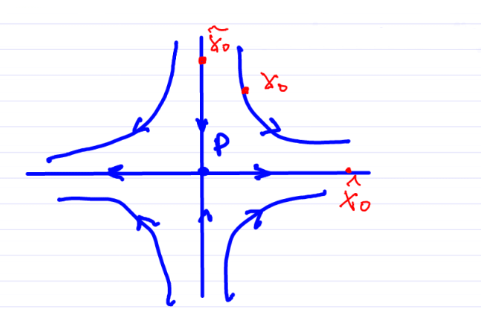
\includegraphics[width=0.3\textwidth]{figures/ch4/6limset_ex_1.png}
		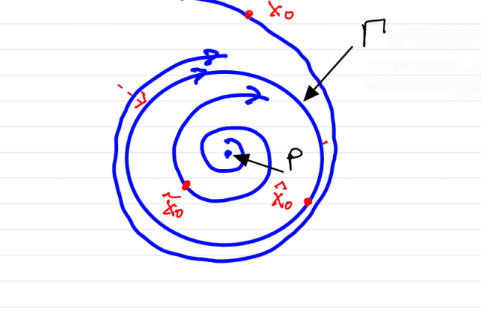
\includegraphics[width=0.3\textwidth]{figures/ch4/6limset_ex_2.png}
		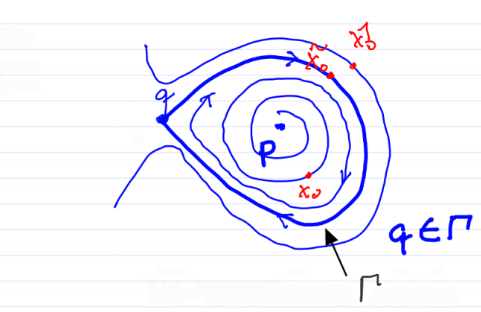
\includegraphics[width=0.3\textwidth]{figures/ch4/6limset_ex_3.png}
		\caption{Three example systems for which we examine the respective limit sets. The arrows labelled $\Gamma $ denote a stable limit cycle (middle) and a homoclinic orbit (right).}
		\label{fig:limset_ex}
	\end{figure}
	For the leftmost dynamical system we have $\omega(p)=\alpha(p)=\{p\}$ and
\begin{align}
	\omega(x_0) &= \emptyset, \quad &\omega(\tilde{x}_0) &= \{p\}, \quad &{\omega }(\hat{x}_0)&= \emptyset, \\
	\alpha(x_0)&=\emptyset, \quad & \alpha(\tilde{x}_0)&=\emptyset,\quad &\alpha(\hat{x}_0&=\{p\}.
\end{align}
	For the middle dynamical system we have 
\begin{align}
	\omega(x_0) &= \Gamma, \quad &\omega(\tilde{x}_0) &= \Gamma, \quad &{\omega }(\hat{x}_0)&= \Gamma, \\
	\alpha(x_0)&= \textrm{unclear} , \quad & \alpha(\tilde{x}_0)&=\{p\},\quad &\alpha(\hat{x}_0)&=\Gamma.
\end{align}
	For the rightmost dynamical system we have 
\begin{align}
	\omega(x_0) &= \Gamma, \quad &\omega(\tilde{x}_0) &= \{q\}, \quad &{\omega }(\hat{x}_0)&=  \textrm{unclear}, \\
	\alpha(x_0)&= \{p\} , \quad & \alpha(\tilde{x}_0)&=\{q\},\quad &\alpha(\hat{x}_0)&= \textrm{unclear} .
\end{align}
\end{ex}

We now introduce two theorems which give us more insight into these limit sets.
